\documentclass{ltxdoc}
\usepackage{doc}
\usepackage[T1]{fontenc}
\usepackage[utf8]{inputenc}
\usepackage{a4wide}
\usepackage{tikz}
\usepackage[siunitx, RPvoltages]{circuitikz}
\ctikzset{%
    american,
    cute inductors,
}
\usepackage{booktabs}
\usepackage{hyperref}
\hypersetup{colorlinks=true,  % false: boxed links; true: colored links
    linkcolor=blue,           % color of internal links
    urlcolor=blue,            % color of external links
}
\usepackage{showexpl}
\lstset{pos=t, overhang=0pt,hsep=\columnsep,vsep=\bigskipamount,
    rframe=single,numbers=left,numberstyle=\tiny,numbersep=.3em, xleftmargin=1em,
    columns=flexible, language=[LaTeX]TEX,breaklines=true,
    basicstyle=\small\ttfamily,tabsize=3, varwidth}
\usepackage{circledsteps}

\title{The \texttt{circledsteps} package: circled numbers, circled steps and more}
\author{Romano Giannetti <romano.giannetti@gmail.com>}
% when we have lot of insets, this is better:
\parindent=0pt\parskip=6pt plus 6pt minus 2pt\relax

\begin{document}
\maketitle

\section{Introduction}

This package was born thanks to the discussion on \href{https://tex.stackexchange.com/questions/7032/good-way-to-make-textcircled-numbers}{tex.stackexchange.com}, and to the help of the several authors that contributed to the answers. The base idea is to have a command that can create arbitrary ``circled'' text (numbers or letters) and that can work in normal text \textbf{and} in a node in a \texttt{tikzpicure} or derivative. That forbid to use \texttt{Ti\emph{k}Z} itself for the circles --- you can't safely nest \texttt{tikzpictures}s.

This package provides two things: the first one, macros to generate the circled text that use the original \texttt{pict2e} method, and then a (simple, to be taken as an example) set of macro to generate sequential circled numbers that can be referenced afterward.

\section{Basic commands}

The basic commands are:

\begin{tabular}{>{\ttfamily\textbackslash}ll}
    \toprule
    Circled\{\} & circled text using the package colors, text on the baseline\\
    CircledTop\{\} & circled text using the package colors, circle on the baseline\\
    CircledText\{\} & circled text using the current color (may fail\footnotemark in moving arguments)\\
    \bottomrule
\end{tabular}
\footnotetext{in the sense it can select the wrong color.}

The parameters for the output are controlled using \texttt{pgfkeys}; you can change them with \verb|\tikzset|; you can obviously limit the effect of change using normal \LaTeX{} scoping rules.

\begin{tabular}{>{\ttfamily}lll}
    \toprule
    \textbf{Parameter} & \textbf{Meaning} & \textbf{Default value} \\
    \midrule
    /csteps/inner ysep  & vertical spacing & 4pt\\
    /csteps/inner xsep  & horizontal spacing & 4pt\\
    /csteps/inner color & color of the text  & red\\
    /csteps/outer color & color of the circle & blue\\
    \bottomrule
\end{tabular}

The working of the package is better explained with examples.

\begin{LTXexample}
This is normal text: \Circled{1} is on the baseline, \CircledTop{2} is on top.

This is more evident if you have descendents, like p:\Circled{p} and \CircledTop{p}.
\end{LTXexample}


\begin{LTXexample}
For big horizontal things the circle becomes oval: \Circled{200} or \CircledTop{199}.
\end{LTXexample}


\begin{LTXexample}
Inside \texttt{tikz} they work ok:

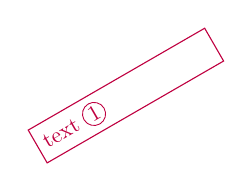
\begin{tikzpicture}[scale=0.8, rotate=30,
    text width=3cm, transform shape]
    \node [draw,color=purple]{text \Circled{1}};
\end{tikzpicture}
\end{LTXexample}


\begin{LTXexample}
\tikzset{/csteps/inner ysep=10pt}
\tikzset{/csteps/inner xsep=10pt}
If you like more breathing space:
\Circled{1}  \Circled{2} \Circled{p} \Circled{200} \Circled{199}.
\par\bigskip
\end{LTXexample}

\begin{LTXexample}
\tikzset{/csteps/inner color=green}
\tikzset{/csteps/outer color=gray}
If you want to change colors it's easy:
\Circled{1}  \Circled{2} \Circled{p} \Circled{200} \Circled{199}.
\par\bigskip
\end{LTXexample}

\begin{LTXexample}
Or even you can have inline numbers like \CircledText{1} or
exponents\textsuperscript{\CircledText{2}} and so on.
\textcolor{red}{They follow the current color:  \CircledText{1} and \CircledText{2} automatically,} as you can see:  \CircledText{$1+1\approx3$}. In-text circled numbers look better when a bit smaller, though, as you can see in {\small\CircledText{1}} for example.
\end{LTXexample}

Notice that \verb|\CircledText{}| uses the special ``\texttt{.}'' color defined by \texttt{xcolor}; when page breaks occurs it can get the wrong color.

No, you can't fill the circle/oval. Pull requests in that sense are welcome.

\section{Automatically generated numbers}

The command \verb|\cstep| will generate a circled number, starting from \texttt{1}, that can be referenced with the normal \verb|\label| mechanism. You can reset the numbering with 
\verb|\startcstep|. For example:

\begin{circuitikz}[scale=0.9, baseline=(VCC), transform shape]
    \draw (0,0)  node[ground](GND){} to[V=$v_s$] ++(0,2)
    to[R, l2^=$R_1$ and \SI{1}{k\ohm}, l2 valign=b] ++(2,0) coordinate(firstb);
    \node [above] at(firstb) {\cstep\label{c:b1}};
    \node [below] at(firstb) {0};
    \draw (firstb) node[npn, anchor=B](Q1){};
    \draw (Q1.E) node[left]{\num{-0.7}\cstep};
    \draw (Q1.C) to[R, l2_=$R_2$ and \SI{5}{k\ohm}, f<=\num{0.93}] ++(0,2.5) 
        node[vcc](VCC){$V_{CC}=\SI{10}{V}$} ;
    \draw (Q1.E) to[R, l2_=$R_3$ and \SI{10}{k\ohm},
    f=\num{0.93}] ++(0,-2.5) node[vee](VEE){$V_{EE}=\SI{-10}{V}$}
        node[left]{\cstep\label{c:ie1}};
    \path (VCC) node[right]{\cstep\label{c:ic1}};
    \draw (Q1.E) -- ++(1,0) coordinate(tmp) to[C=$C_1$] (tmp |- GND) node[ground]{};
    \draw (Q1.C) -- ++(1,0) coordinate(g1) to[short, -o] ++(1,0);
    \node [above] at(g1) {\cstep\label{c:g1}};
    \node [below] at(g1) {\num{5.35}};
\end{circuitikz}\quad
\begin{minipage}[t]{0.5\linewidth}
    %% minipage reset these..
    \parindent=0pt\parskip=6pt plus 6pt minus 2pt\relax
    \ref{c:b1} let's neglect (to be confirmed!) $I_B$, $V_B\approx\SI{0}{V}$;\par
    \ref{c:ie1} $I_{E1_Q}=(V_{E1_Q}-V_{EE})/R_3$;\par
    \ref{c:ic1} $I_{C1_Q} \approx\SI{0.93}{mA}$;\par
    \ref{c:g1} $V_{CC}-R_2I_{C2_Q}= \SI{5.35}{V}$; $V_{CE1_Q}=\SI{6.05}{V}$;\par
\end{minipage}



\lstinputlisting{ctikzexample.tex}

\bigskip

\section{Personalize it!}

The definition of \verb|CircledTexT| is simply the following one; you can get idea and define your own easily (beware of spaces at the end of the lines, though!): 

\begin{lstlisting}
\newcommand{\CircledText}[1]{%
    \begingroup
    \tikzset{/csteps/inner color=., /csteps/outer color=.}%
    \Circled{#1}%
    \endgroup
}
\end{lstlisting}


Also the implementation of the \verb|\cstep| command and relatives is quite simple, and you can play a lot with it to change things (formats, colors, the type of numbering, and so on):

\begin{lstlisting}
\newcounter{cstepcnt}
\newcommand{\startcstep}{\setcounter{cstepcnt}{0}}
\newcommand{\resetcstep}{\setcounter{cstepcnt}{0}}
\newcommand{\cstep}{%
    \refstepcounter{cstepcnt}%
    \Circled{\scriptsize\arabic{cstepcnt}}%
}
\renewcommand{\thecstepcnt}{\textbf{\arabic{cstepcnt}:}}
\end{lstlisting}


\end{document}
